\section{Simulation Analysis}
\label{sec:simulation}

For the simulation we used NGSpice was used.

An ideal transformer model was used, by implementing a dependent current source and a dependent voltage source. 

The values of n (dependent sources dependency parameter), the resistance and the capacitance were adjusted during the preparation of the assignment in order to achieve
the maximum accuracy of the desired output voltage.

in Figure~\ref{fig:sim3a} we can see the input voltage of the dependent voltage source, Vr, the output voltage of the envelope detector, V(4), and the output voltage of the voltage regulator, V(5).


\begin{figure}[h] \centering
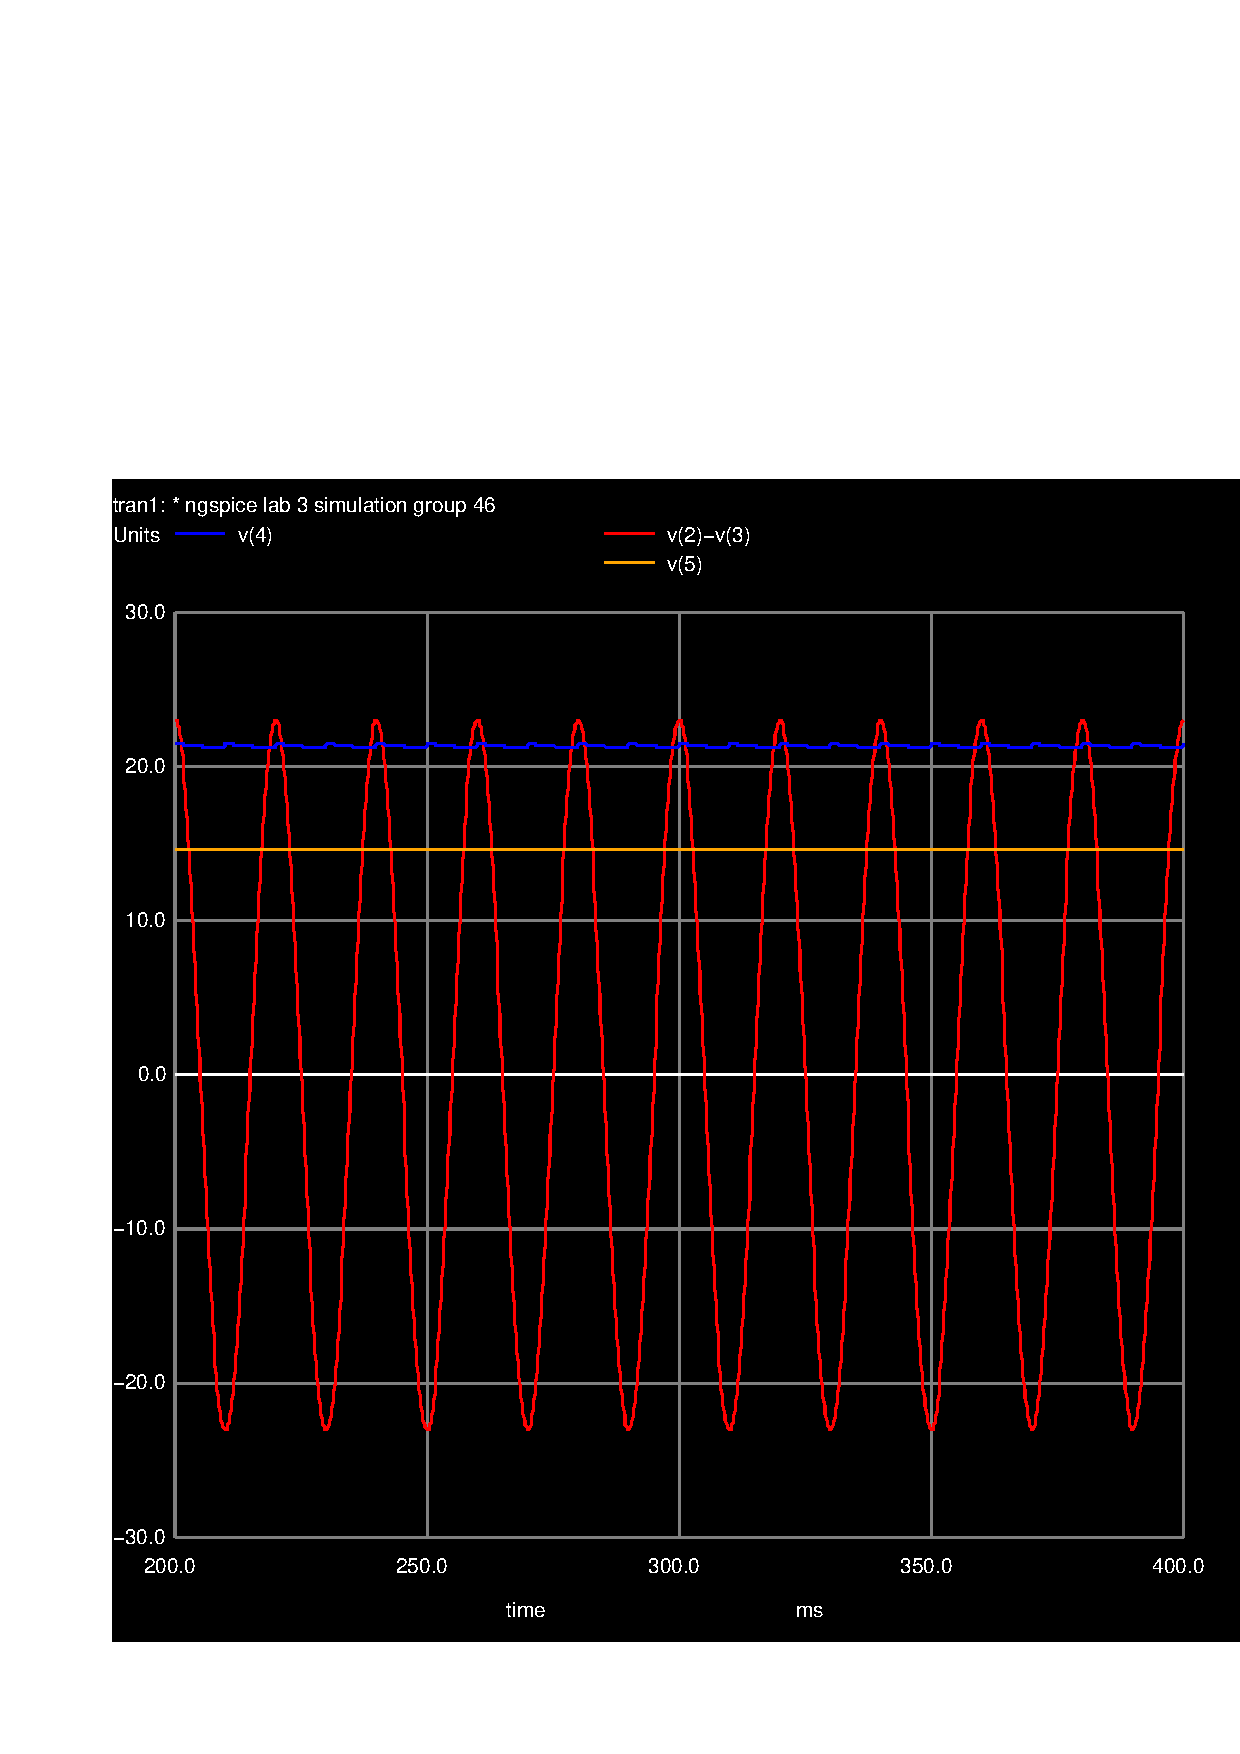
\includegraphics[width=0.6\linewidth]{sim3a.pdf}
	\caption{Plot of the computed voltages}
\label{fig:sim3a}
\end{figure}


Here we can see the effect of the envelope and voltage regulators. As anticipated in the Theoretical Analysis, the first decreases the ripple voltage and 
the second keeps the output voltage constant. Even if V(5) is not a perfect DC voltage (we can note some oscillations, which are expectedm, due to the non-linear behavior of the diodes), $V(5) - 12V$ is 
very close to zero, which is what is expected in a real life rectifier and the goal of the lab. 

As we can see in Figure~\ref{fig:sim3b}, the regulated ripple voltage is far less than the envelope ripple voltage, which indicates that the circuit is operating as expected. 

\begin{figure}[h] \centering
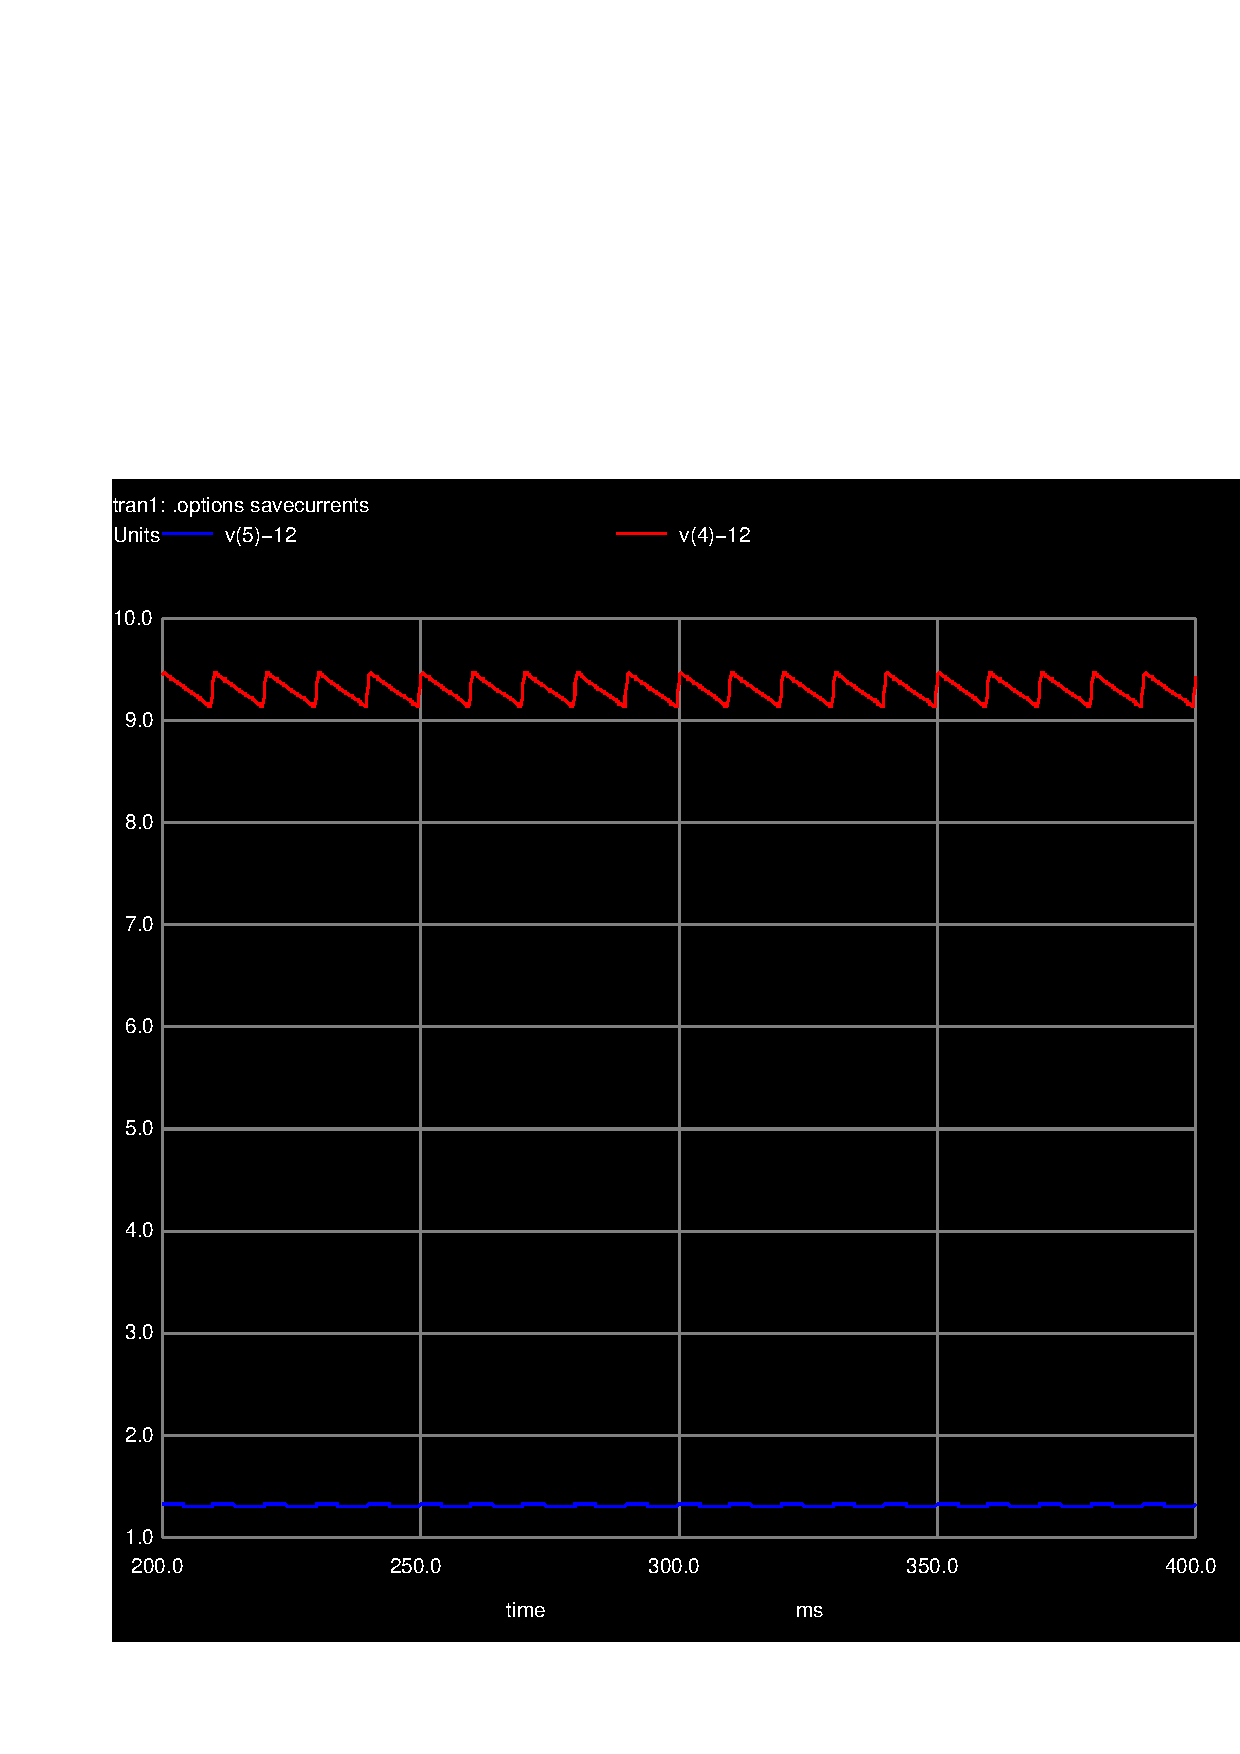
\includegraphics[width=0.6\linewidth]{sim3b.pdf}
	\caption{$v(4)-12V$, $v(5)-12V$}                        
\label{fig:sim3b} 
\end{figure}

The following tables show various values of interest:

\begin{table}[h]
        \parbox{.45\linewidth}{
  \centering
  \begin{tabular}{|l|r|}
    \hline
    {\bf Name} & {\bf Value [V]} \\ \hline
    maximum(v(4))-minimum(v(4)) & 1.741797e-01\\ \hline
mean(v(4)) & 1.276542e+01\\ \hline

  \end{tabular}
  \caption{Envelope ripple and average voltages.}
	\label{tab:env}
}
\hfill
        \parbox{.45\linewidth}{
  \centering
  \begin{tabular}{|l|r|}
    \hline
    {\bf Name} & {\bf Value [V]} \\ \hline
    maximum(v(5))-minimum(v(5)) & 1.933408e-02\\ \hline
mean(v(5)) & 1.331470e+01\\ \hline

  \end{tabular}
  \caption{Regulator ripple and average voltages.}
  \label{tab:reg}
}
\end{table}






